%! Author = joels
%! Date = 27/01/2022

\section{Semantische Analyse}
\textbf{$\rightarrow$ Kümmert sich um die semantische Analyse}\\
\textbf{Input:} Syntaxbaum (konkret oder abstrakt)\\
\textbf{Output:} Abstrakter Syntaxbaum + Symboltabelle

\subsection{Semantische Prüfung}
\textbf{Prüfe, dass das Programm gemäss Sprchregeln Sinn macht.}
\begin{itemize}[topsep=0pt]
    \itemsep -0.2em
    \item Deklarationen
    \SubItem{Jeder Identifier ist eindeutig deklariert}
    \item Typen
    \SubItem{Typregeln sind erfüllt}
    \item Methodenaufrufe
    \SubItem{Argumente und Parameter sind kompatibel}
    \item Weitere Regeln
    \SubItem{z.B. Keine zyklische Vererbung, nur eine main()-Methode}
\end{itemize}
\textbf{Benötigte Informationen:}
\begin{itemize}[topsep=0pt]
    \itemsep -0.2em
    \item Deklarationen: Variablen, Methoden, Klassen
    \item Typen:
    \SubItem{Vordefinierte Typen (int, boolean etc.)}
    \SubItem{Benutzerdefinierte Typen (Klassen)}
    \SubItem{Arrays}
    \SubItem{Typ-Polimorphismus (Vererbung)}
\end{itemize}

\subsection{Symboltabelle}
\textbf{Datenstruktur zur Verwaltung der Deklarationen.}\\
\textbf{Wiederspiegelt hierarchische Bereiche im Programm.}\\
$\rightarrow$ Global Scope einführen, um mehrere Klassen zu managen.\\
\textbf{Shadowing:} Deklarationen in inneren Bereichen verdecken gleichnamige von äusseren Bereichen.\\
\textbf{Hiding:} Base Klasse und Sub Klasse haben beide die Variable x deklariert. $\rightarrow$ Sub Klasse muss mit super auf x von Base zugreifen.\\
\begin{minipage}{0,5\linewidth}
    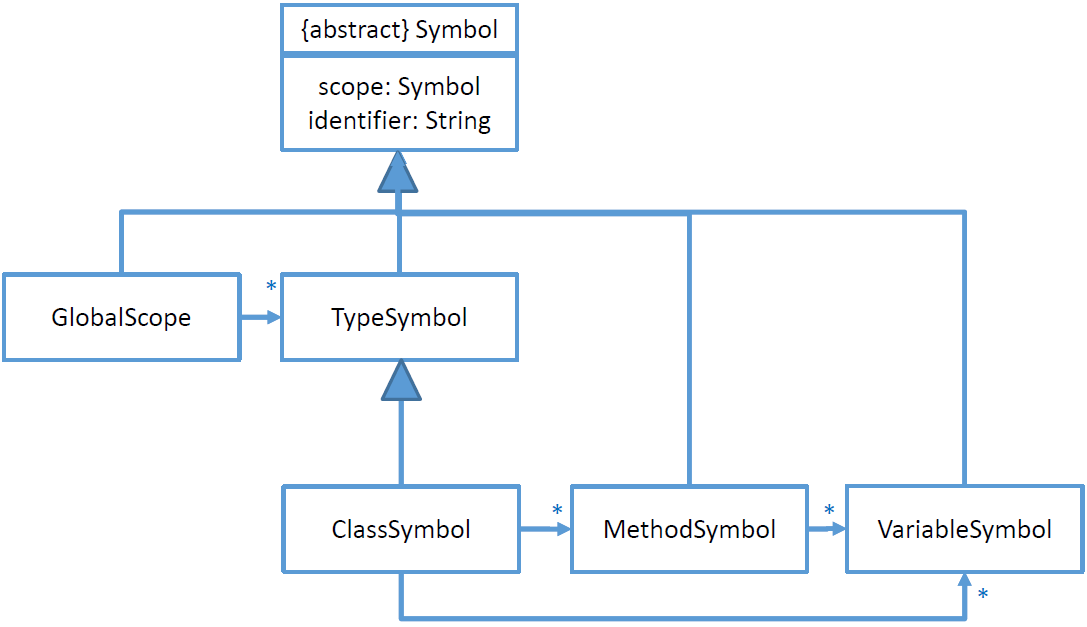
\includegraphics[width=\linewidth]{symbol_table}
\end{minipage}
\begin{minipage}{0,5\linewidth}
    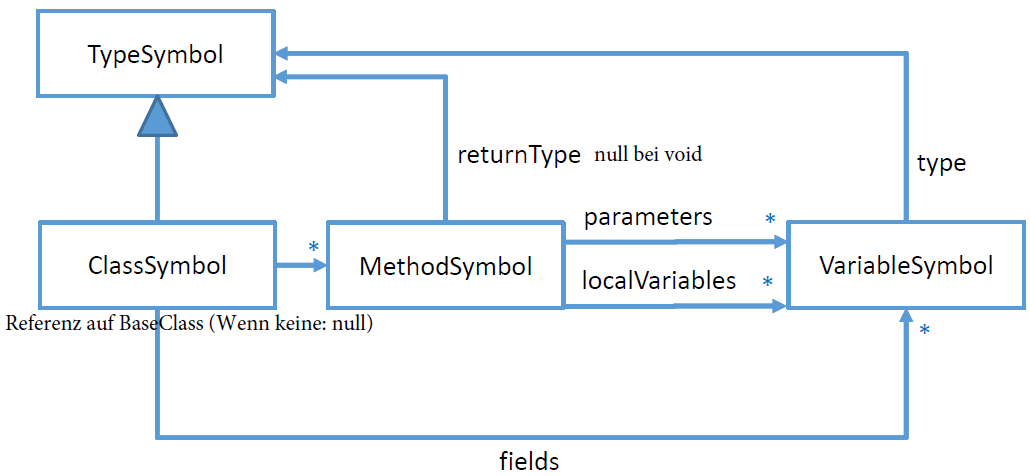
\includegraphics[width=\linewidth]{symbol_table_detail}
\end{minipage}

\subsubsection{Besonderheiten}
\begin{itemize}[topsep=0pt]
    \itemsep -0.2em
    \item Vordefinierte Types: int, boolean, string
    \SubItem{Als Inbuild Type in Global Scope einfügen}
    \item Vordefinierte Konstanten: true, false, null, this
    \SubItem{true, false, null als Konstanten in Global Scope}
    \SubItem{null ist Poly-Typ (kompatibel zu allen Referenztypen)}
    \SubItem{this speziell bei Analyse behandeln}
    \item Vordefinierte Methoden: writeString etc.
    \item Vordefinierte Variablen: length
    \SubItem{Nur für Array-Typen, ist read-only}
\end{itemize}

\subsection{AST verknüpfen}
\textbf{Symboltabelle enthält Mapping Symbol $\rightarrow$ AST}\\
\begin{minipage}{0,5\linewidth}
    \subsubsection{1. Konstruktion der Symboltabelle}
    \textbf{AST traversieren:}
    \begin{itemize}[topsep=0pt]
        \itemsep -0.2em
        \item Beginne mit Global Scope
        \item Pro Klasse, Methode, Parameter, Variable:
        \SubItem{Symbol in übergeordnetem Scope einfügen}
        \item Explizit und/oder mit Visitor Pattern
    \end{itemize}
    \textbf{Forward-Referenzen: Typ-Namen und Designatoren noch nicht auflösen}
\end{minipage}
\begin{minipage}{0,5\linewidth}
    \subsubsection{2. Typen bei Symbolen auflösen}
    \begin{itemize}[topsep=0pt]
        \itemsep -0.2em
        \item Für Variablentyp, Parametertyp, Rückgabetyp etc.
        \item Brauche Suche für Identifier auf Symboltabelle
        \item Welches Symbol deklariert Identifier \dq id\dq?
        \SubItem{Suche beim innerstem Scope beginnen}
    \end{itemize}
\end{minipage}
\textbf{Suchfunktion:}
\begin{lstlisting}
Symbol find(Symbol scope, String identifier) {
    if (scope == null){ return null; } // Über global scope hinaus
    for (Symbol declaration: scope.allDeclarations()) {
        if (declaration.getIdentifier().equals(identifier)) {
            return declaration;
        }
    }
    return find(scope.getScope(), identifier); //Rekursiv in nächst höheren Bereich
}
\end{lstlisting}
\begin{minipage}{0,5\linewidth}
    \subsubsection{3. Deklarationen in AST auflösen}
    \begin{itemize}[topsep=0pt]
        \itemsep -0.2em
        \item Traversiere Ausführungscode in AST (Method Body)
        \item Jeden Designator auflösen (Deklaration zuordnen)
    \end{itemize}
    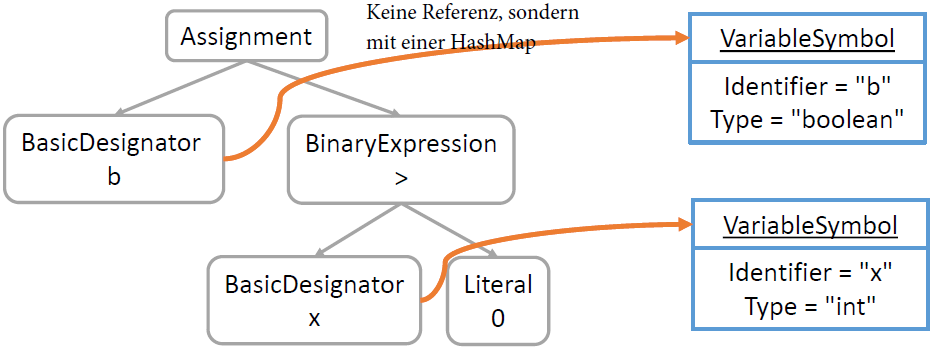
\includegraphics[width=\linewidth]{deklaration_in_ast}
\end{minipage}
\begin{minipage}{0,5\linewidth}
    \subsubsection{4. Typen in AST bestimmen}
    \begin{itemize}[topsep=0pt]
        \itemsep -0.2em
        \item Typ zu jeder Expression zuordnen
        \SubItem{Literal: definierter Typ}
        \SubItem{Designator: Typ der Deklaration}
        \SubItem{Unary/Binary Expression: Resultat des Operators}
    \end{itemize}
    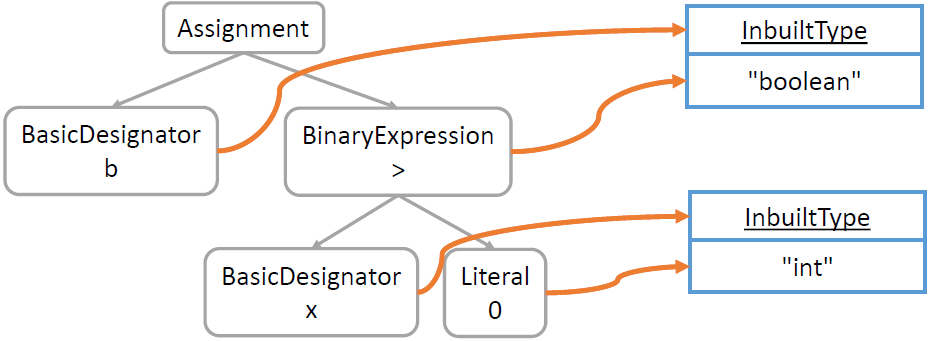
\includegraphics[width=\linewidth]{typen_in_ast}
\end{minipage}

\subsection{Semantic Checks}
\begin{itemize}[topsep=0pt]
    \itemsep -0.2em
    \item Alle Designators beziehen sich auf Variablen/Methoden
    \item Typen stimmen bei Operationen
    \item Kompatible Typen bei Zuweisung
    \item Argumentliste passt auf Parameterliste
    \item Bedingung in if, while sind boolean
    \item Return-Ausdruck passt
    \item Keine Mehrfachdeklarationen
    \item Kein Identifier ist reserviertes Keyword
    \item Exakt eine main()-Methode
    \item Array Length ist read-only
\end{itemize}
\begin{lstlisting}
@Override
public void visit(BinaryExpressionNode node) {
    Visitor.super.visit(node); // post-order traversal
    var leftType = symbolTable.findType(node.getLeft());
    var rightType = symbolTable.findType(node.getRight());

    switch (node.getOperator()) {
        case PLUS -> {
            // error(), falls Type nicht int ist
            checkType(leftType, globalScope.getIntType());
            checkType(rightType, glbalScope.getIntType());
            symbolTable.fixType(node, GlobalScope.INT_TYPE);
        }
    }
}
\end{lstlisting}